
In this section we consider the dynamics of \eqref{eq:magnetichamiltonian} for $b\gg 0$, that is, in the case where KAM and perturbative methods are not readily applicable. With no clear battle plan, we approach the question in an exploratory way: we look for (quasi)-periodic orbits, consider their stability, and see where stability is missing. To this end, we prove the existence of a Poincar\'e section, later we induce ``coarse'' symbolic dynamics and apply the Lempel-Ziv complexity to make sense of the dynamics. What we find is rich dynamics and a visual method of analysis well suited for similar problems.

The phase space of our system is $\mathbb R^2\times\mathbb R^2$, however we can reduce the phase space to a Poincar\'e section as follows:
\begin{proposition}
Let $S$ be the union of discs of radius $R$ centered at $\mathbb Z^2+1/2$. The sets $\Sin$ and $\Sout$ defined as:
\begin{align}
\label{def:poincaresectionIN}
\Sin &= \bigcup_{x\in\partial S} \{x\} \times \{v\in\mathbb R^2 : v\cdot (x-1/2) < 0\},\\
\label{def:poincaresectionOUT}
\Sout &= \bigcup_{x\in\partial S} \{x\} \times \{v\in\mathbb R^2 : v\cdot (x-1/2) > 0\},
\end{align}
are Poincar\'e sections for the system \eqref{eq:magnetichamiltonian}.
\end{proposition}
We prove this in a later subsection. This greatly helps visualize long term behavior, since the magnitude of the velocity of a trajectory is constant. Furthermore, we can pass the system to the torus, which reduces $S$ to one disc. So, when plotting we only need two dimensions: one to parametrize $\partial S$ and another for the velocity.

\subsection{First impressions and lots of quasiperiodicity}

For the remainder of this section we fix $R=1/3$ and $\|p\|=1$. In \ref{fig:periodicorbits}

\begin{figure}[!th]
\centering
\begin{subfigure}{0.49\textwidth}
\centering
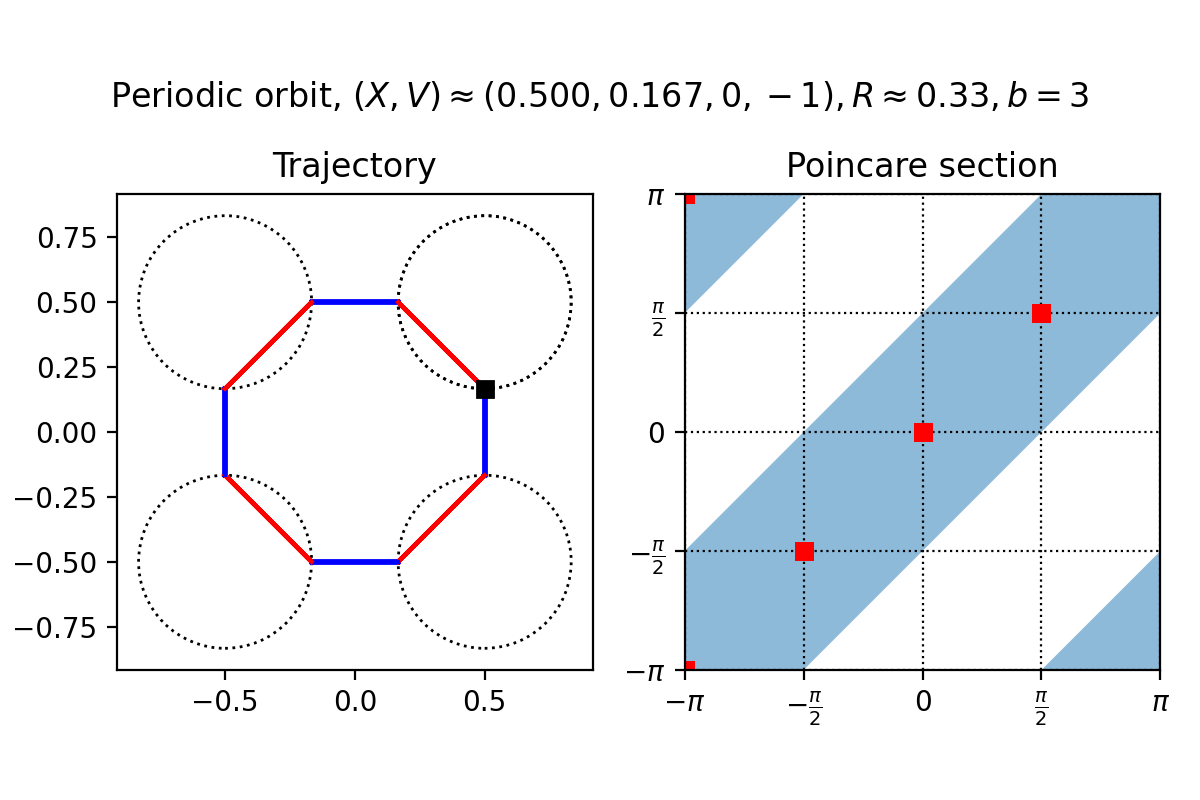
\includegraphics[width=\textwidth, trim={0 1cm 0 1cm}, clip]{stable_square_with_poincare.png}
\caption{say smth albert}
\label{subfig:periodicorbit1}
\end{subfigure}
%
\begin{subfigure}{0.49\textwidth}
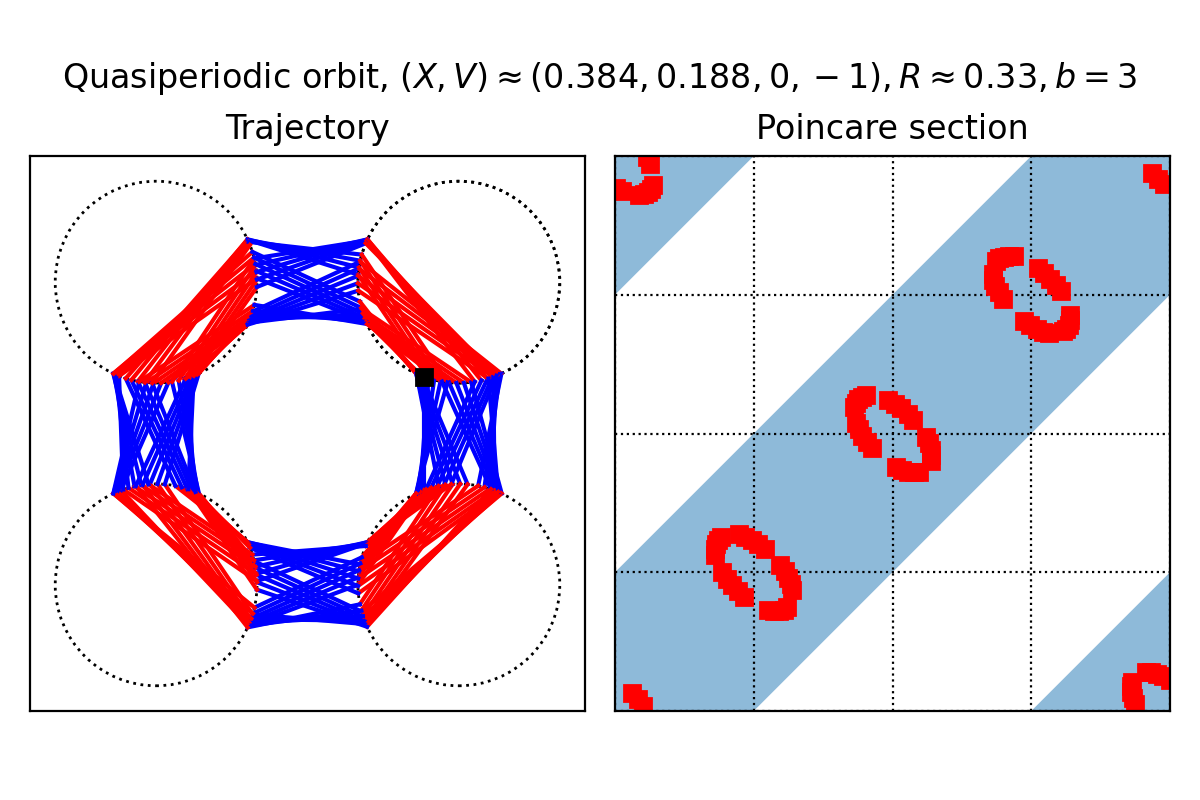
\includegraphics[width=\textwidth, trim={0 1cm 0 1cm}, clip]{perturbed_stable_square_with_poincare.png}
\caption{say smth albert}
\label{subfig:periodicorbit2}
\end{subfigure}
%
\begin{subfigure}{0.49\textwidth}
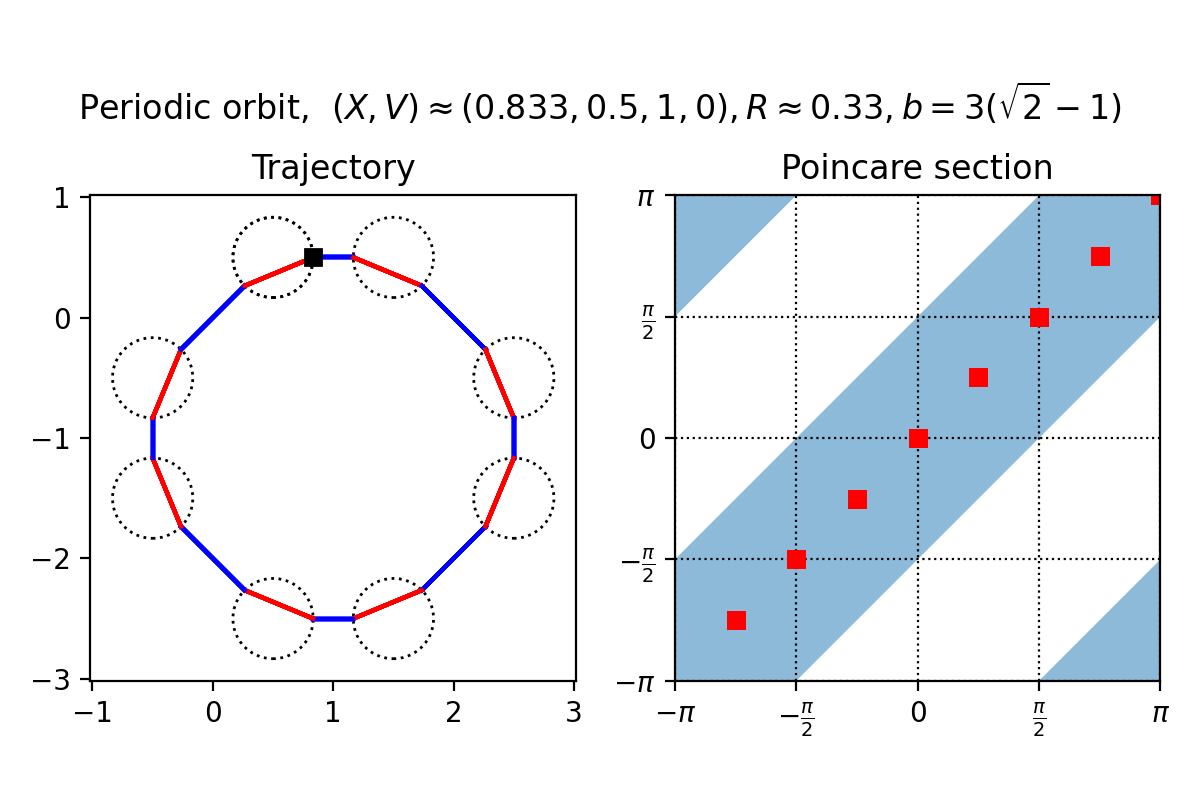
\includegraphics[width=\textwidth, trim={0 1cm 0 1cm}, clip]{stable_octagon_with_poincare.png}
\caption{a.}
\label{subfig:periodicorbit3}
\end{subfigure}
%
\begin{subfigure}{0.49\textwidth}
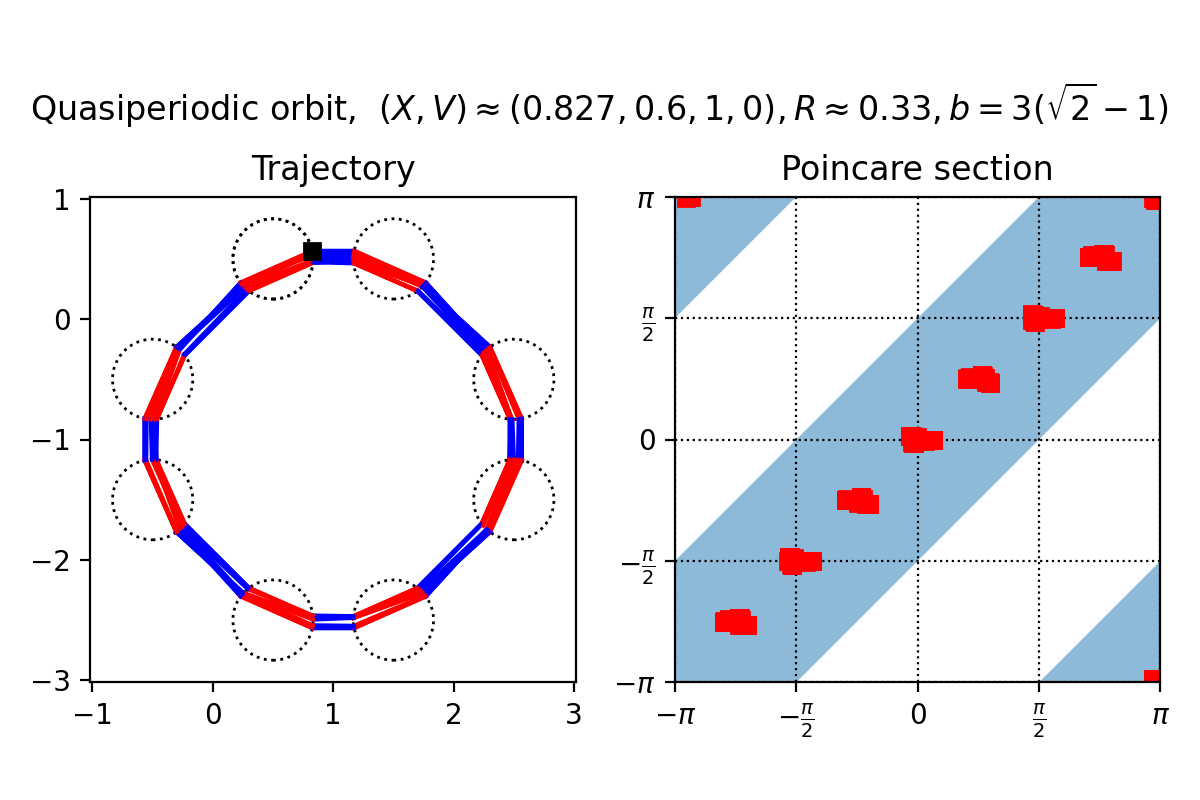
\includegraphics[width=\textwidth, trim={0 1cm 0 1cm}, clip]{perturbed_stable_octagon_with_poincare.png}
\caption{.}
\label{subfig:periodicorbit4}
\end{subfigure}
%
\begin{subfigure}{0.49\textwidth}
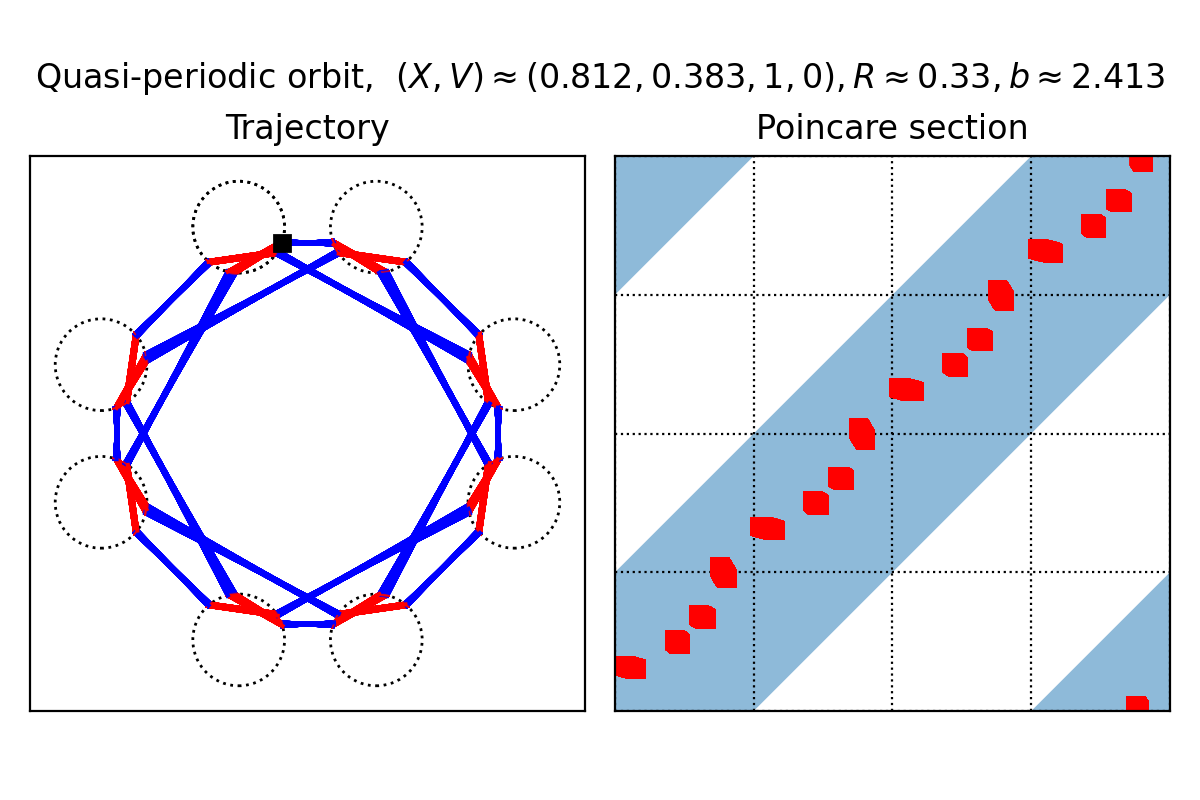
\includegraphics[width=\textwidth, trim={0 1cm 0 1cm}, clip]{star_with_poincare.png}
\caption{.}
\label{subfig:periodicorbit5}
\end{subfigure}
%
\begin{subfigure}{0.49\textwidth}
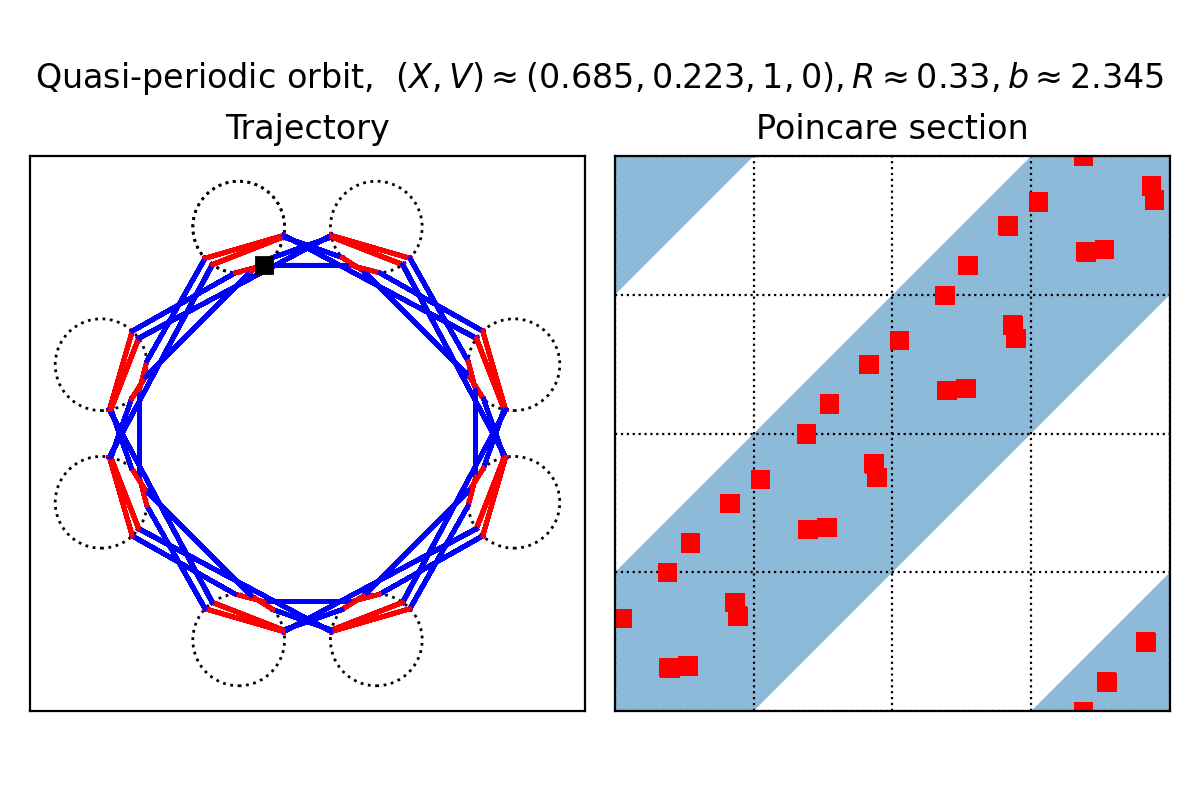
\includegraphics[width=\textwidth, trim={0 1cm 0 1cm}, clip]{doubled_star_with_poincare.png}
\caption{.}
\label{subfig:periodicorbit6}
\end{subfigure}
%
\begin{subfigure}{0.49\textwidth}
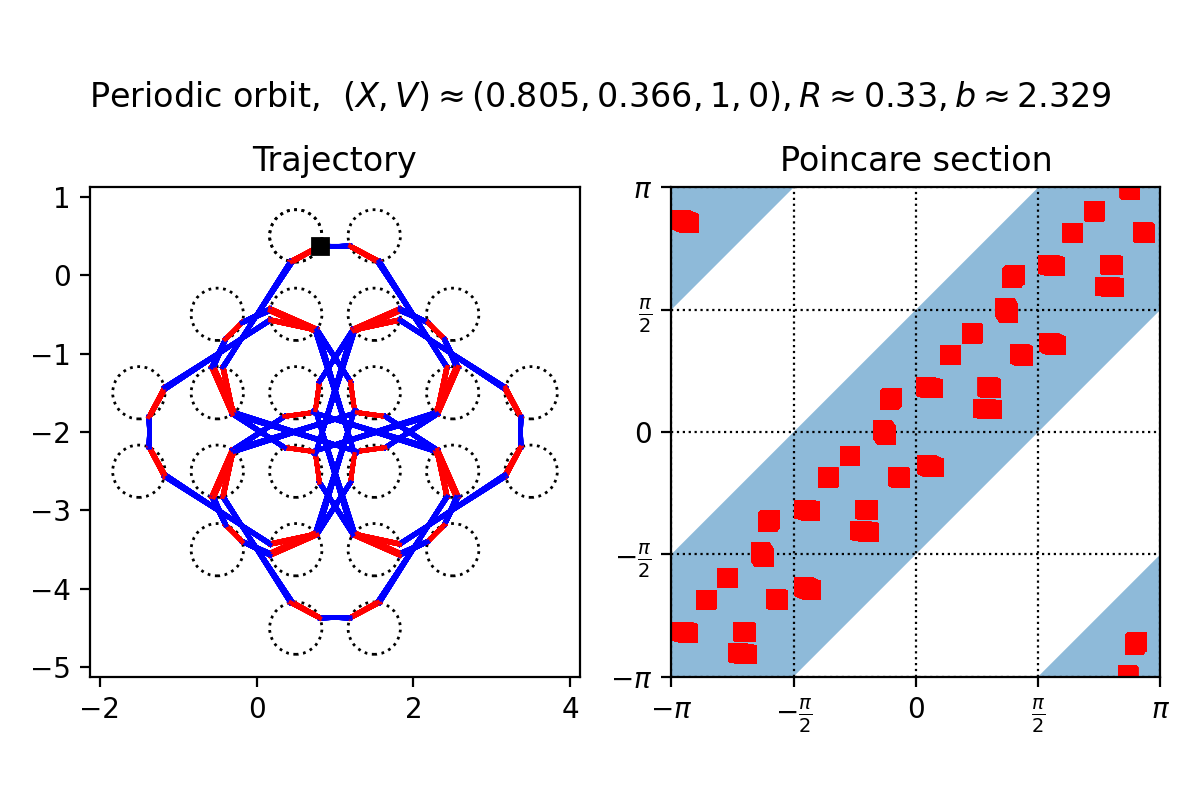
\includegraphics[width=\textwidth, trim={0 1cm 0 1cm}, clip]{sophisticated_with_poincare.png}
\caption{.}
\label{subfig:periodicorbit7}
\end{subfigure}
%
\begin{subfigure}{0.49\textwidth}
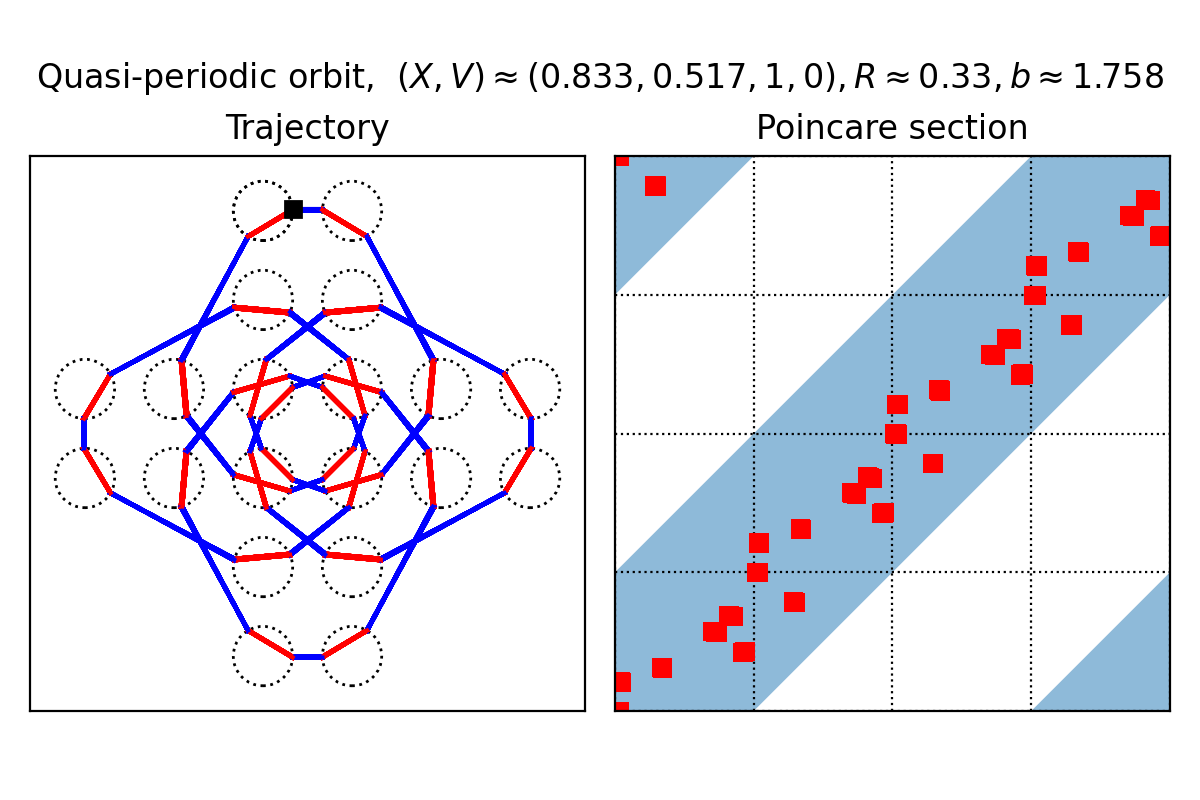
\includegraphics[width=\textwidth, trim={0 1cm 0 1cm}, clip]{distinguished_with_poincare.png}
\caption{.}
\label{subfig:periodicorbit8}
\end{subfigure}
%
\begin{subfigure}{0.49\textwidth}
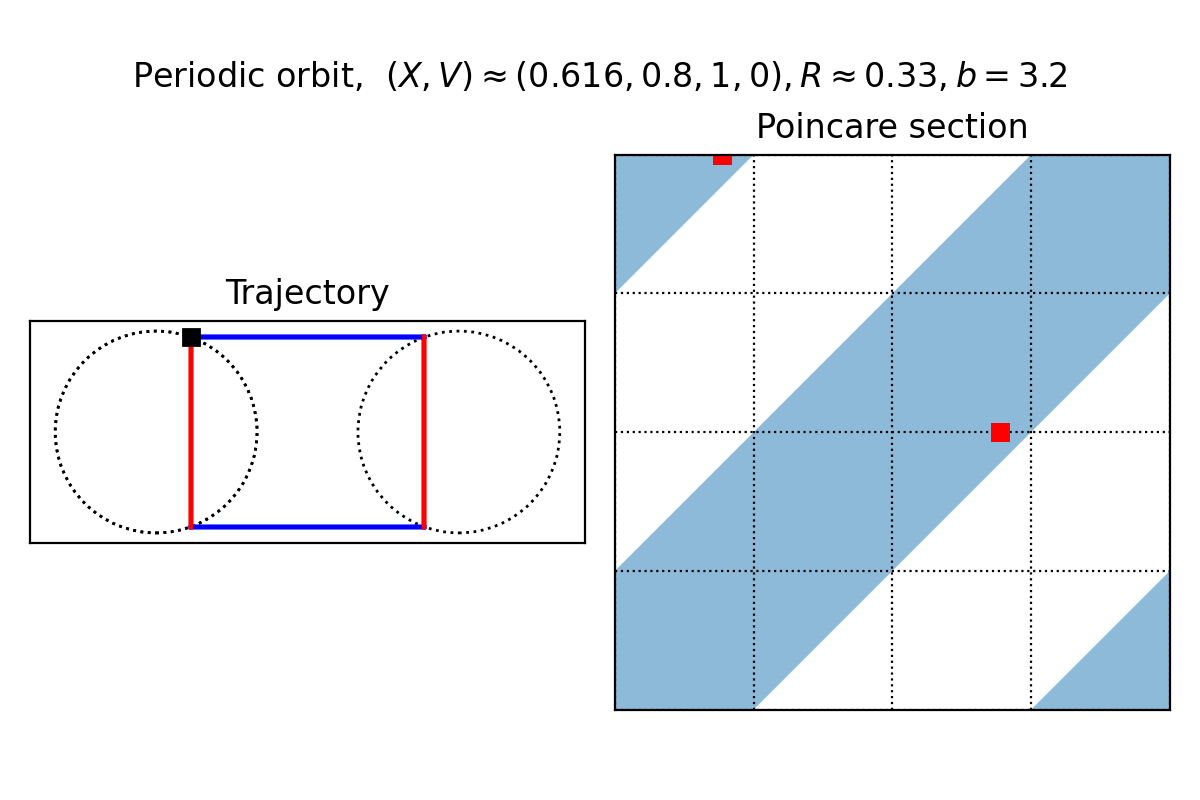
\includegraphics[width=\textwidth, trim={0 1cm 0 1cm}, clip]{unstable_square_with_poincare.png}
\caption{.}
\label{subfig:periodicorbit9}
\end{subfigure}
%
\begin{subfigure}{0.49\textwidth}
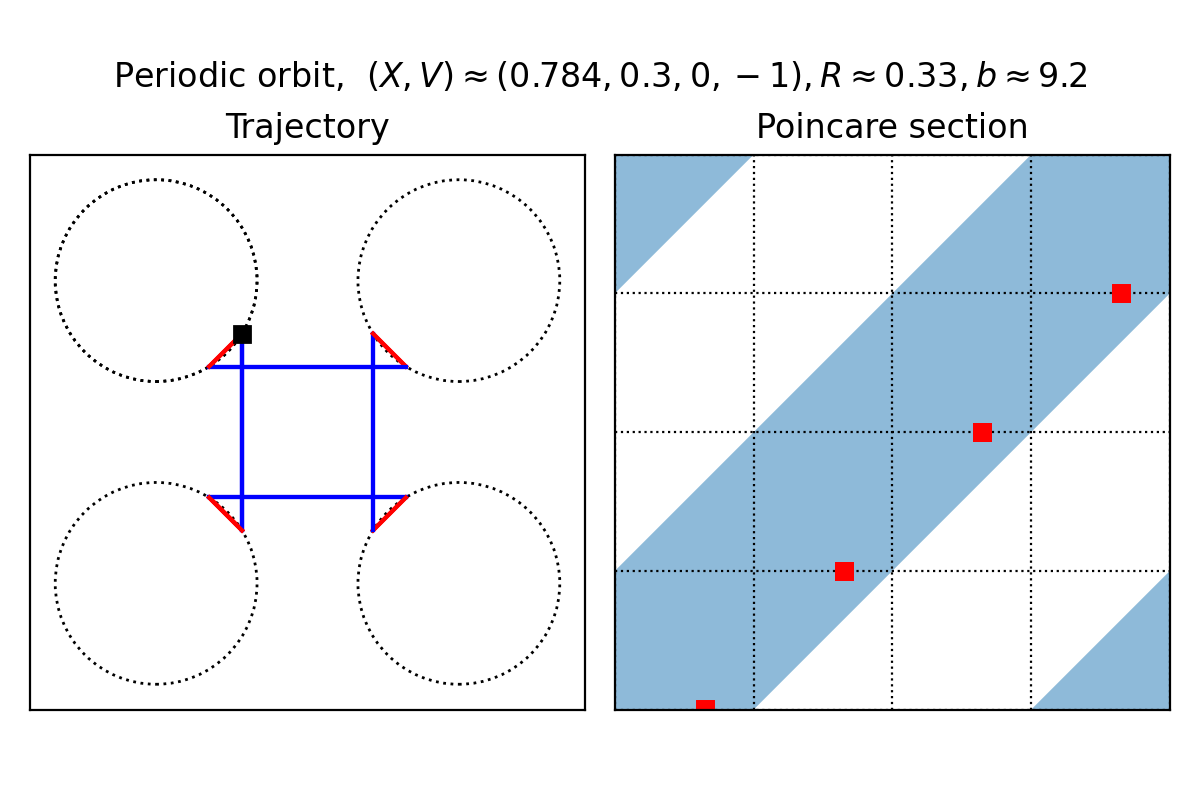
\includegraphics[width=\textwidth, trim={0 1cm 0 1cm}, clip]{unstable_loopy_square_with_poincare.png}
\caption{.}
\label{subfig:periodicorbit10}
\end{subfigure}
\caption{Examples of (quasi)-periodic for varying choices of parameters.}
\label{fig:periodicorbits}
\end{figure}


\begin{figure}[!th]
\ContinuedFloat
\centering
\begin{subfigure}{0.49\textwidth}
\centering
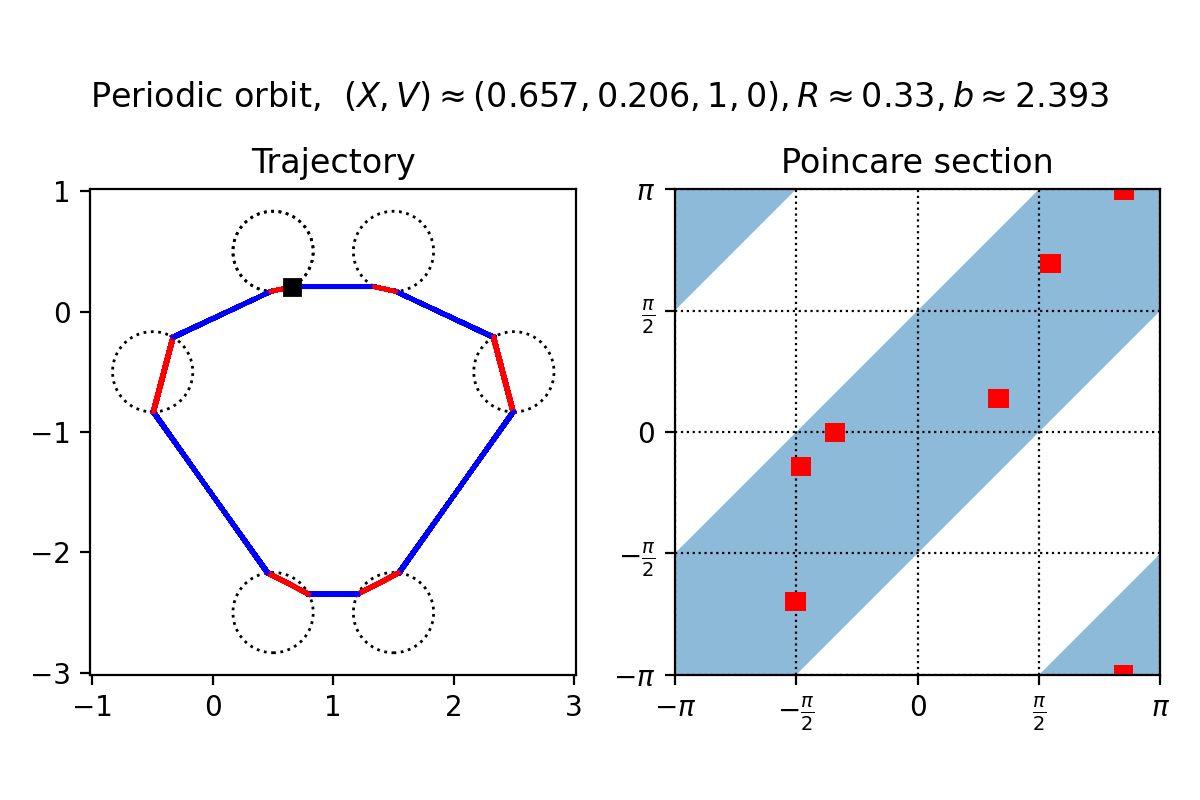
\includegraphics[width=\textwidth, trim={0 1cm 0 1cm}, clip]{lopsided_octagon_with_poincare.png}
\caption{say smth albert}
\label{subfig:periodicorbit11}
\end{subfigure}
%
\begin{subfigure}{0.49\textwidth}
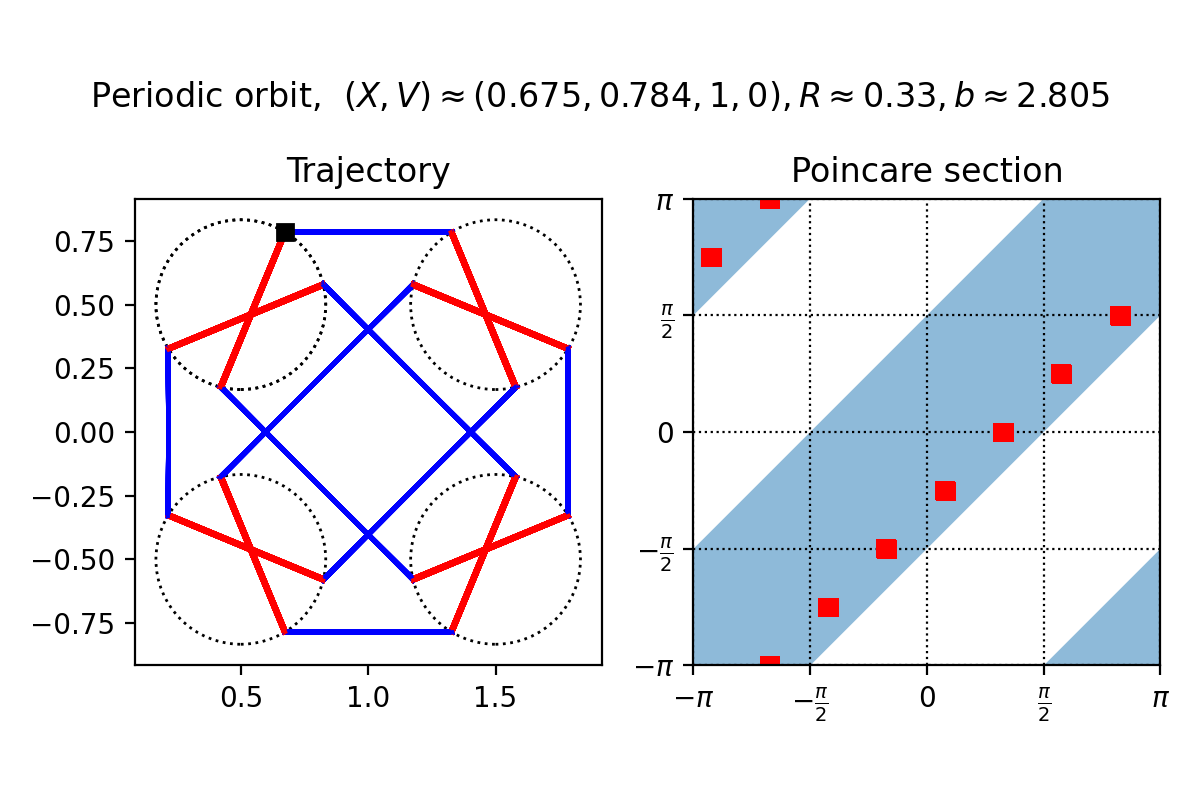
\includegraphics[width=\textwidth, trim={0 1cm 0 1cm}, clip]{strange_square_with_poincare.png}
\caption{.}
\label{subfig:periodicorbit12}
\end{subfigure}
%
\begin{subfigure}{0.49\textwidth}
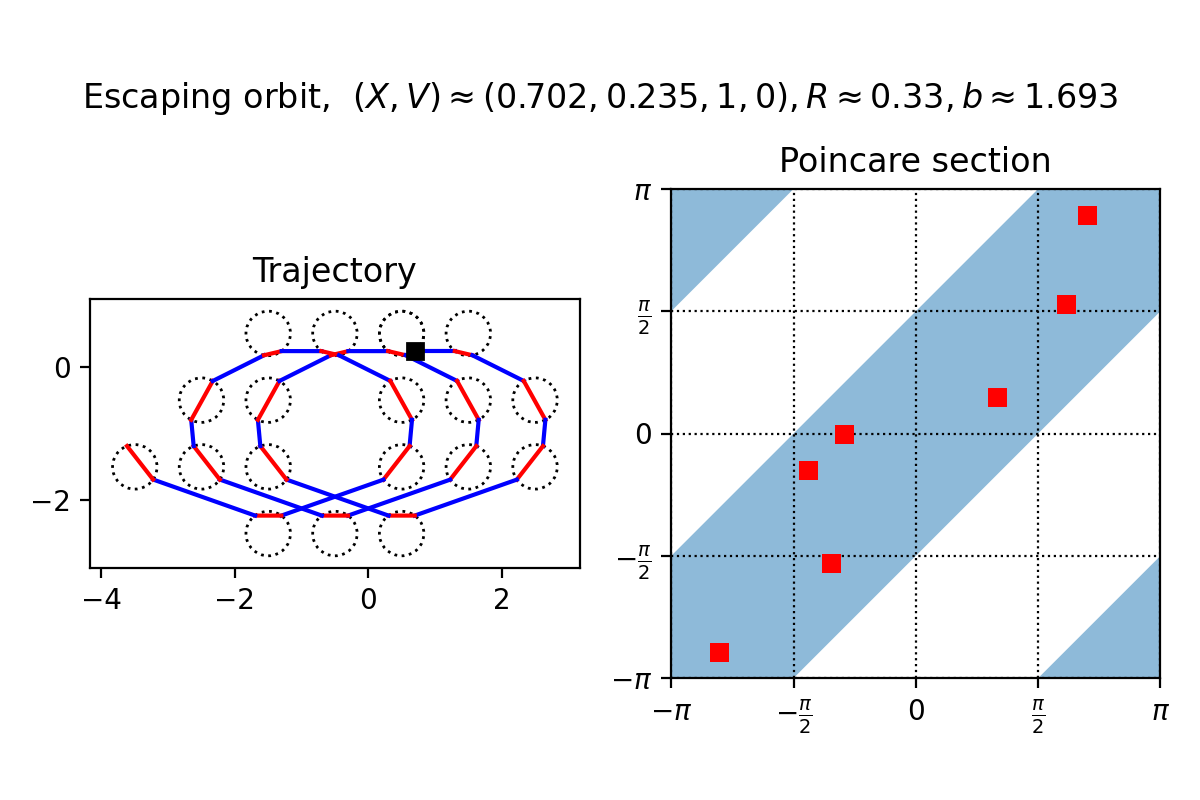
\includegraphics[width=\textwidth, trim={0 1cm 0 1cm}, clip]{walker_with_poincare.png}
\caption{.}
\label{subfig:periodicorbit13}
\end{subfigure}
%
\begin{subfigure}{0.49\textwidth}
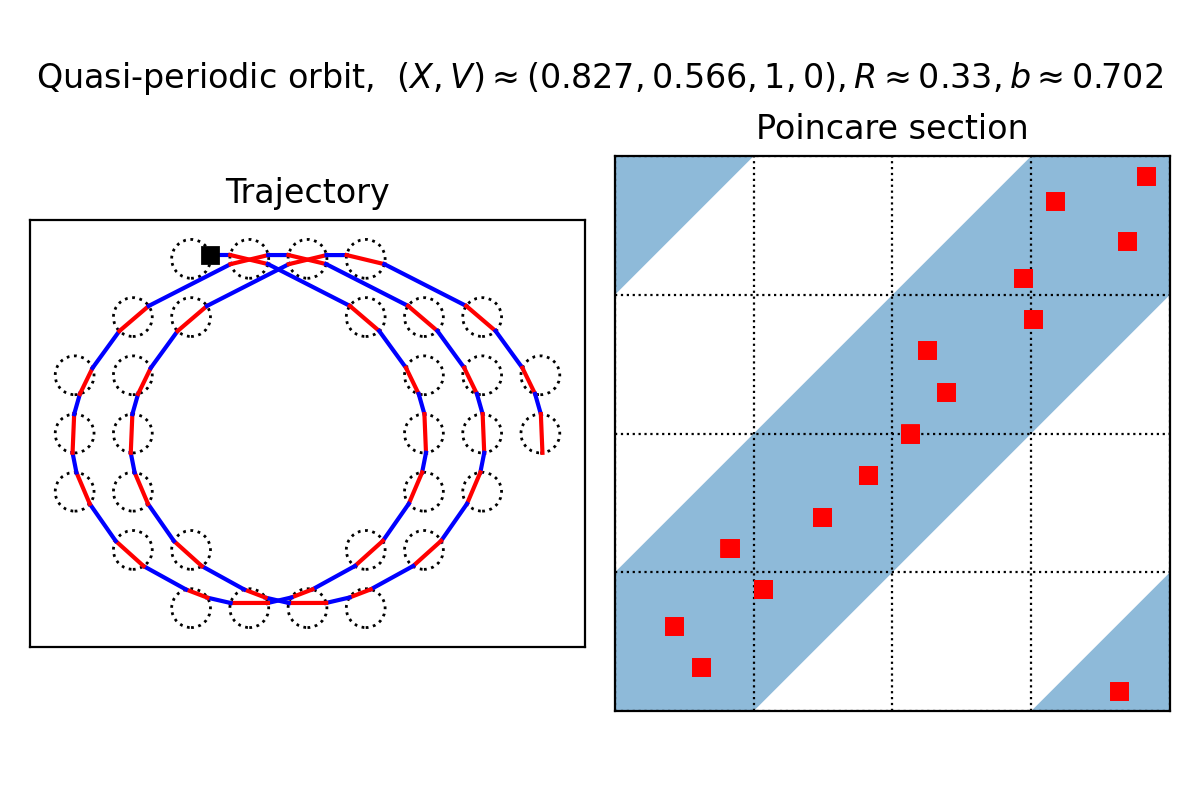
\includegraphics[width=\textwidth, trim={0 1cm 0 1cm}, clip]{big_walker_with_poincare.png}
\caption{.}
\label{subfig:periodicorbit14}
\end{subfigure}
%
\begin{subfigure}{0.49\textwidth}
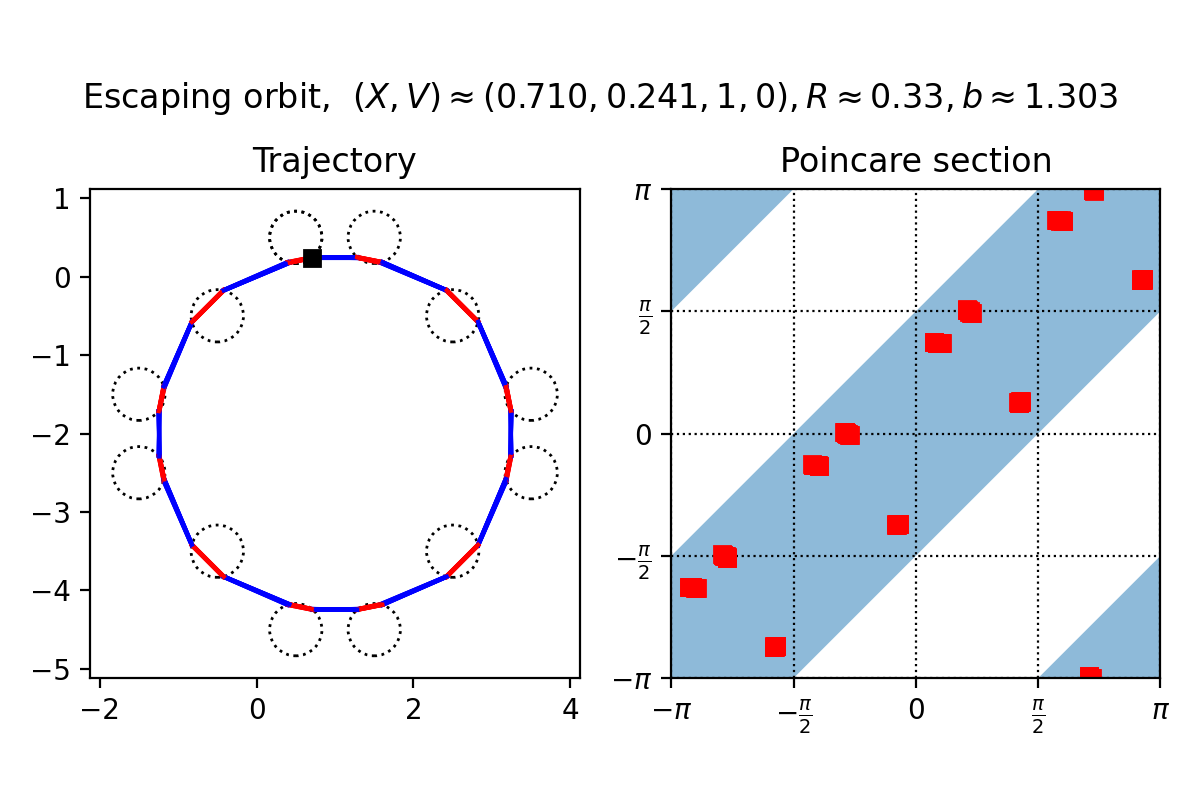
\includegraphics[width=\textwidth, trim={0 1cm 0 1cm}, clip]{12gon_with_poincare.png}
\caption{.}
\label{subfig:periodicorbit15}
\end{subfigure}
%
\begin{subfigure}{0.49\textwidth}
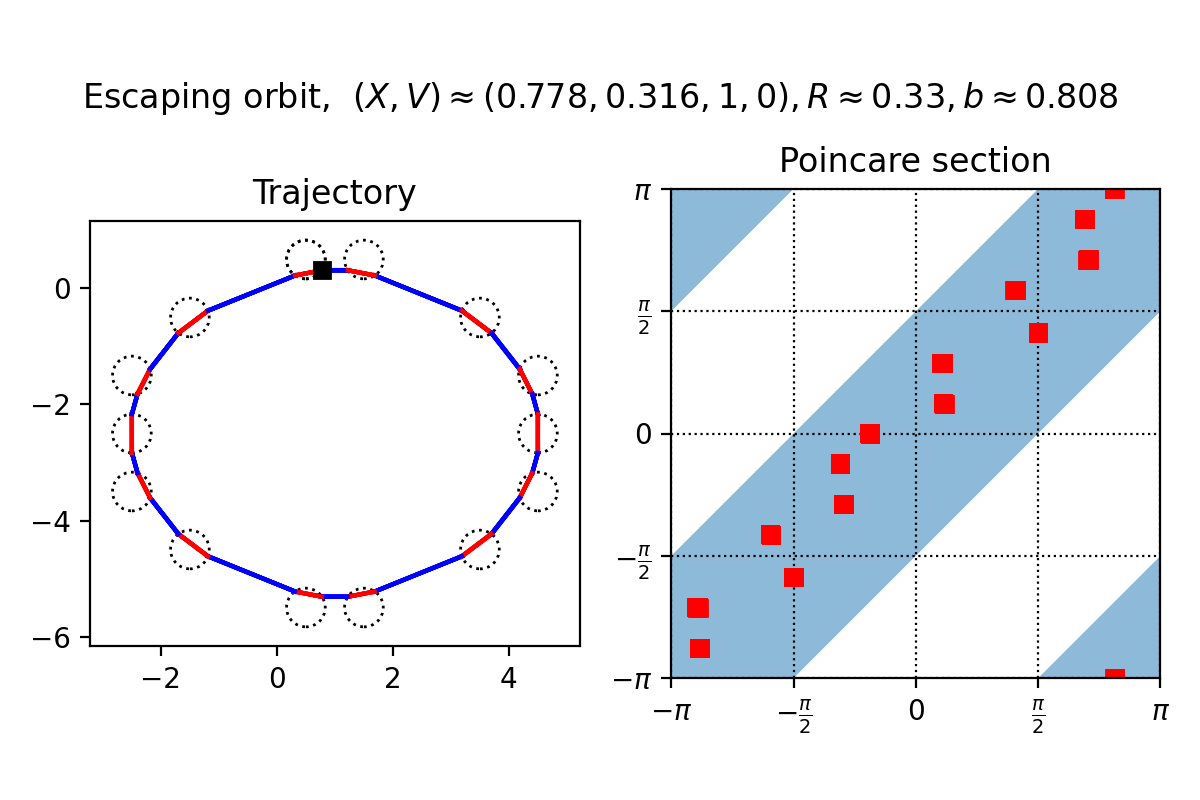
\includegraphics[width=\textwidth, trim={0 1cm 0 1cm}, clip]{egg_with_poincare.png}
\caption{.}
\label{subfig:periodicorbit16}
\end{subfigure}
%
\begin{subfigure}{0.49\textwidth}
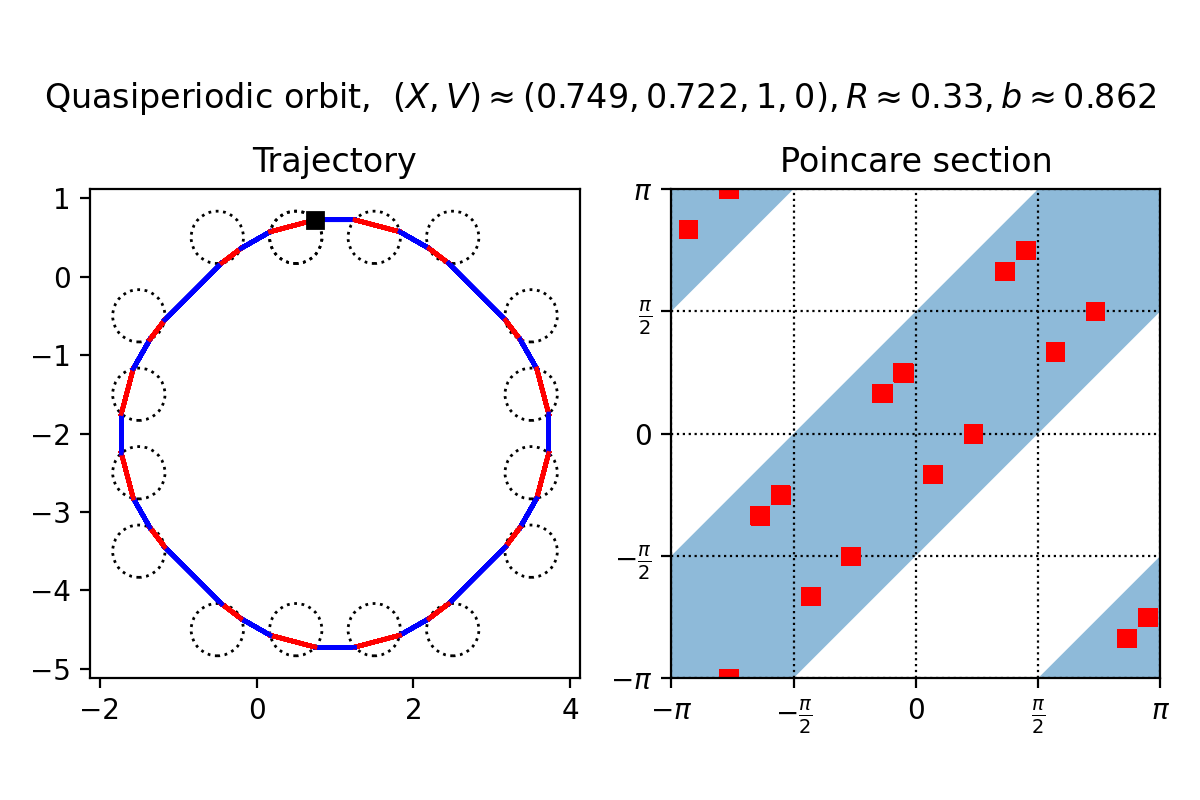
\includegraphics[width=\textwidth, trim={0 1cm 0 1cm}, clip]{big_square_with_poincare.png}
\caption{.}
\label{subfig:periodicorbit17}
\end{subfigure}
%
\begin{subfigure}{0.49\textwidth}
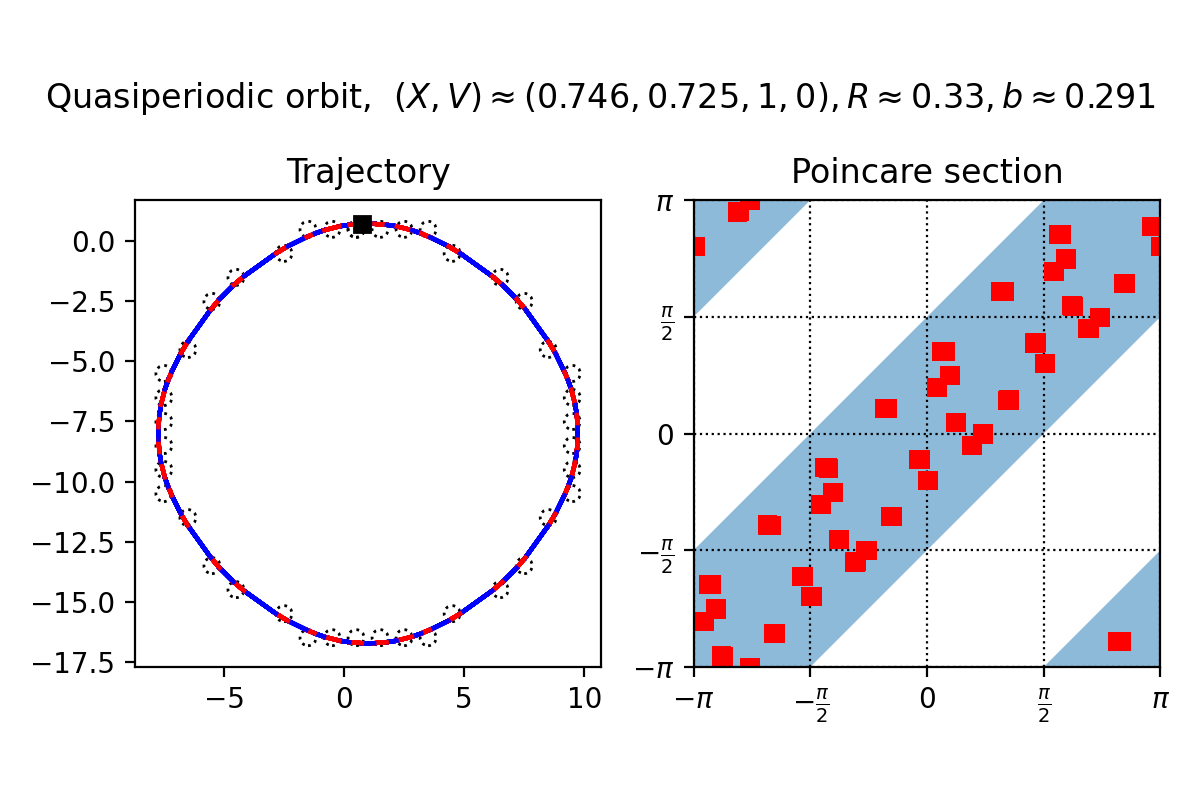
\includegraphics[width=\textwidth, trim={0 1cm 0 1cm}, clip]{big_circle_with_poincare.png}
\caption{.}
\label{subfig:periodicorbit18}
\end{subfigure}
\caption{Examples of (quasi)-periodic for varying choices of parameters.}
\label{fig:periodicorbits1}
\end{figure}

\subsection{Constructing a Poincar\'e section}

\begin{lemma}
The flow of \eqref{eq:magnetichamiltonian} induces a well-defined map $P_\text{io}:\Sin\to\Sout$.
\end{lemma}
\begin{proof}
Let $(x,v)\in \Sin$, under the flow of \eqref{eq:magnetichamiltonian} we know the Larmor circle $C$ with initial conditions $(x,v)$ intersects $\partial S$ in $x$ and that at $x$ the circles are not tangential. Two circles intersecting at a point non-tangentially must intersect at a second point, so there exists $x\neq y\in\partial S\cap C$. By the flow of \eqref{eq:magnetichamiltonian} there must also exist a velocity $w\in\mathbb R^2$ such that $w\cdot(x-1/2)>0$, that is $(y,w)\in\Sout$. Hence we have $P_\text{io}(x,v) = (y,w)$. 
\end{proof}

We can say more, there exists a line $\ell$ through the center $a$ of the Larmor circle $C$ and the center $(1/2,1/2)$ of $\partial S$. The two circles are symmetric with respect to the reflection $T$ with respect to $\ell$. This means $Tx=y$, and $Tv = -w$. The following statement is more interesting.

\begin{lemma}\label{lem:SoutToSin}
The flow of \eqref{eq:magnetichamiltonian} induces a well-defined map $P_\text{oi}:\Sout\to\Sin$.
\end{lemma}
\begin{proof}
Let $(x,v)\in\Sout$, then under the flow of \eqref{eq:magnetichamiltonian} we see linear motion. Ignoring the presence of $S$, we see that depending on $v$, the trajectory is either periodic or is dense in $\mathbb T$.

Focusing on the first case, in finite time we return to the point $x$. Since the trajectory is a line $\ell$ interesecting $\partial S$ transversally, there must be another point of intersection $x\neq y\in\partial S\cap\ell$. The velocity at $y$ must also be $v$, so due to the geometry of a circle, $(y,v)\in\Sin$. For the second case, we can pick $\varepsilon>0$ such that all points in $U=(\partial S\cap B_\varepsilon(x))\times\{v\}\subset \Sout$ are transversal to $\partial S$. Let $(y,v)\in U$, since the flow is dense for the velocity $v$, ignoring $S$, we know that in finite time the point $(x,v)$ comes to $(y,v)$. The rest of this case follows the same way as previously. 

In either case, the $(y,v)$ we find is not necessarily the first time we enter $\Sin$ but since the number of such points is countable, we can pick the first one $(y_0,v)$, hence, $P_\text{oi}(x,v) = (y_0,v)$ is a well-defined map.
\end{proof}

Now, we can finalize the Poincar\'e map.



Notice that the reasoning is independent of the radius of $S$, nor does it depend on the exact position of $S$. Pulling back to the plane with an infinite number of disks, we can then generalize the setup. Consider a fundamental finite set $A$ of disks where each disk in $A$ can have a different magnetic strength and radius and the disks need not be regularly placed. The above result holds for configurations of disks which can be decomposed as a tiling of such a set $A$.

In \cite{Knauf_2017} a similar result is proved for a configuration of finitely many bumps. In that case a different method was used that did not rely on an infinite number of bumps, in ours the reasoning was simplified due to this.

With the Poincar\'e map we can study the stability of (quasi)-periodic trajectories of the system for a choice of parameters. In \cref{fig:periodicorbits} we provide some examples we constructed using analytic geometry. In \cref{subfig:periodicorbit1} we see a periodic trajectory and its corresponding orbit in the Poincar\'e section. In \cref{subfig:periodicorbit2} we shift the initial condition slightly and see that the orbit in \cref{subfig:periodicorbit1} displays stable behavior. We provide a proof using symbolic algebra in \hl{HERE}. The same can be said comparing \cref{subfig:periodicorbit3} and \cref{subfig:periodicorbit4}. On the other hand, in \hl{add plots with unstable periodic orbit} we have a periodic trajectory that does not seem to be stable.

Constructing periodic trajectories and judging their stability by checking numerically is a reliable approach, however it is limited, since we need a good guess to start with. Uncovering more elaborate (quasi)-periodic behavior in this manner becomes impractical, so we need a tool that can help us single out good candidates ahead of time. We discuss this in the next section.


%The code written in \texttt{Python} utilizes the symbolic algebra system \texttt{Sympy} to define functions, compute derivatives, compose functions, and compute eigenvalues of a Jacobian symbolically. That way we avoid a considerable amount of computation by hand but still retain a high degree of precision when computing numerical values. For long enough periodic orbits, the computation time using symbolic algebra becomes unreasonable, so we require a different way to analyse stability. A common alternative is to compute Lyapunov exponents of the original system or of the Poincar\'e map. However, these approaches are prone to numerical instability and require significant preparation beforehand. We would like to analyze stability from the trajectory directly, and we attempt this via symbolic dynamics in the next section.


%With $B_r(q)\subset \mathbb R^2$ denote the closed ball of radius $r>0$ centered at $q\in\mathbb R^2$. Pick $S=\cup_{N\in\mathbb Z^2}B_{1/3}(N-1/2)$, that is, $S$ is the union of closed balls of radius $1/3$ centered at points of the form $(n-1/2,m-1/2)$ for $n,m\in\mathbb Z$.
%
%The choice of radius $r=1/3$ is arbitrary, we fix it for convenience. Furthermore, we notice the speed of the particle is constant, since $\|X'(0)\|=Rb$, so again for simplicity we fix $\|X'(0)\|=1$. This also fixes the Larmor radius $R=1/b$. A different choice of $r\in (0,1/2)$ and $\|X'(0)\|\in(0,\infty)$ clearly gives rise to different dynamics, however we make the assumption that the dynamics will not differ \textit{qualitatively}, i.e., in any case we expect to find periodic orbits, chaotic behavior, and the methods we use for studying these are still valid.
%
%Hence, we study the influence of varying the parameter $b>0$ on the above defined system. What we see is four ranges of behavior:
%\begin{enumerate}
%\item For values $b\approx0$ we can approximate the dynamics as a perturbation of a system with no magnetic field at all,
%\item For a range of ``small'' values of $b$, the dynamics are similar to that of a uniform field in $\mathbb R^2$,
%\item there is an intermediate range where both stable and unstable periodic dynamics occur
%\item there exists a value $b_t$, such that all values $b>b_t$ give rise to unstable dynamics.
%\end{enumerate}
%
%We can use this to already find some simple periodic orbits. We describe one such orbit now.
%
%Let $\delta\in(0,1/3)$ and consider the initial condition $(x,p) = (0,1/2+delta,1,0)$, the trajectory can be seen in \cref{subfig:periodicorbit1}. We can compute that for the choice $b=1/\delta$, the trajectory will be a periodic orbit.
%
%Already, we see that periodic orbits exist for arbitrarily large $b$. It can be shown using Poincar\'e sections that this family of periodic orbits is unstable.
%
%Another family of periodic orbits are given for $\delta\in(-1/\sqrt{18},1/3)$, where the initial condition is $(x,p)=(0,1/2+\delta,1,0)$ and $b = 1/(\delta+\sqrt{1/9-\delta^2})$
%
%Another family of periodic orbits are given for $\delta\in(1/\sqrt{18},1/3)$, where the initial condition is $(x,p)=(0,1/2+\delta,1,0)$ and $b = 1/(\delta-\sqrt{1/9-\delta^2})$
%
%Lastly, we have a more complicated periodic orbit that forms an octagon for 


